%!TEX program = xelatex
\documentclass[a4paper, 12pt]{report}
\usepackage{xeCJK, geometry, fontspec}
\usepackage[backend=biber,style=numeric,sorting=none]{biblatex}
%-----------------------------------------------------
\setCJKmainfont{教育部標準楷書}
\setmainfont{Times New Roman}
\linespread{1.5}
\geometry{margin=2cm}
\setlength{\parindent}{2em}
\bibliography{main.bib}
%-----------------------------------------------------
\title{
	{\Huge 肉類食品新鮮度監測系統}\\
	{\bf Monitoring System of Freshness of Meat}\\[2cm]
	{國立中山大學資訊工程學系}\\
	{110 學年度大學部專題製作競賽}\\[2cm]
}
\author{
	{Arthor: 李銘庭 (B073040005), 伍建瑋 (B073040008), 蔡孟師 (B073040019)}\\[1cm]
	{Advisor: 賴威光}
}
\date{}

\begin{document}
	\maketitle
	\chapter*{摘要}
\addcontentsline{toc}{chapter}{摘要}

本次專題預期將製作一可收納食物,並在食物腐敗、散發不良氣味之前,能夠感測出來
並即時通知的裝置,藉此避免造成使用者在不清楚食物已經腐敗的狀況下進行食用。
首先,不同的食物腐敗時散發出的化學成分不盡相同,因此我們打算先以偵測肉類食品
為出發點進行實作,肉類食品之所以放久了會腐敗產生惡臭味,是因為肉品中的微生物在
生長時所產生化學物質,如假單胞菌分解蛋白質,所產生硫化物,如硫化氫(H2S)、氨氣(NH3)、
硫醇等等的化合物,而這類分解作用,也就是俗稱的「腐敗」,藉由能夠偵測先前提到的腐敗時
所產生的氣體的氣體感測元件收集到的數據,來判斷該肉品是否可以繼續食用,順利的話
將增加不同種類的食物判斷標準,且考慮更多不同食物腐敗時可能產生的其他變化特性。
例如:pH值、水份含量等等來判斷是否繼續食用。 
	\tableofcontents
	\chapter{簡介}

\section{新鮮程度判定}
平常在廚房中,如果是明顯腐敗有異味,或是剛買回來的新鮮肉類食材,都能明顯決定是否要拿來吃。
但有時仍會疑惑,有些放了一段時間,可能外表還保持乾淨,但是觸感有點不太一樣。或者看似有很小部份異常,
不確定是否損壞,整個食物丟掉又覺得很可惜時,就很希望有存在一個實際能判斷的儀器或方法來解決問題。

\section{腐敗的特徵}\footnote{\url{https://read01.com/zh-tw/58Exkm.html#.YWknDS3RZQI}}
腐敗狀況的判定大致可以藉由觀察顏色變深、表面黏稠度、彈性、產生的異味氣體的程度決定。
色澤的部分,新鮮的肉表面有光澤,多呈紅色或淡紅色,且顏色均勻。但隨著存放時間的延長,由於肌紅蛋白被氧化,肉色會逐漸變成紅褐色。顏色越深,可食性越低。而當肉表面變成灰色或灰綠色,甚至出現白色或黑色斑點時,說明微生物已經產生大量的代謝產物,這樣的肉就可能已經不適合食用了。
黏稠度方面,新鮮的肉外表微乾或濕潤,切面稍潮濕,用手摸有油質感,但不發黏。而肉變質以後,由於微生物大量滋生,會產生黏性代謝產物,造成肉表面發黏,甚至出現拉絲。肉類表面發黏是腐敗開始的特徵。
至於彈性,新鮮的肉質地緊密且富有彈性,用手指按壓凹陷後會立即復原。但存放越久,肉裡面的蛋白質、脂肪會逐漸被酶分解,肌纖維被破壞,所以肉會失去原有的彈性,手指壓後的凹陷不僅不能完全復原,甚至會留有痕跡。
最後在氣味方面,新鮮肉具有正常的肉味,而變質的肉由於蛋白質、脂肪、碳水化合物被微生物分解,會產生各種胺類、酸類、酮類等物質,進而產生明顯的腐臭味。

\section{預計研究問題}
\begin{itemize}
	\item 確認「機器測試」是否比「人的鼻子」靈敏或者準確?
		能否實際拿來作為分析食物新鮮度的輔助器具?
	\item 定義與量化本次探討主題「腐敗」的判定,以方便日後實驗描述。
	\item 由於腐敗的特徵眾多,因此我們選擇以最為客觀且容易量化的「氣味」層面著手研究,嘗試檢測與肉類腐敗相關的氣體濃度,並判斷其關聯程度的高低。
		最後總和出一個兼具有效率(成本低,時間少)且精準的判斷模型。
	\item 透過模型設計出相關的硬體設備。
\end{itemize}

	\chapter{相關應用}

\section{電子鼻}
\subsection{人類嗅覺的限制}
即使在現代科技中,依然有許多行業需要依靠人體的嗅覺作為判斷依據。曾經有人做過
一個紅酒實驗 \cite{hodgson_2008} ,他觀察了許多種紅酒,發現同一種紅酒在兩次
紅酒競賽獲得的成績,其相關性不高。此外,人體的感官也可能因為感官疲勞而產生誤差。
因此,依靠人類的感官作為判斷依據的可靠度值得懷疑。
\subsection{原理}
電子鼻是一種用來模擬鼻子功能的電子儀器。利用多個感測器組合而成的一個整體,
而氣體在接觸到電子鼻時,內部的每個感測器會產生不同程度的電阻變化,因此透過
比對不同變化,即可產生電子指紋圖(electronic fingerprint)並辨識出
此為何種氣體,更甚者可計算出該氣體濃度。 \footnote{\url{https://scitechvista.nat.gov.tw/Article/C000003/detail?ID=e1893f7f-9eda-4ed7-ada0-dc226bfc1d57}}
\subsection{應用}
隨著科技演進,越來越多技術可以應用在電子鼻上。舉例來說,人工智慧可以運用
在電子鼻上, \footnote{\url{https://case.ntu.edu.tw/blog/?p=36043}}
\begin{figure}[H]
	\centering
	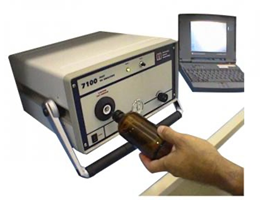
\includegraphics[width=0.5\textwidth]{../../pic/nose.png}
\end{figure}

\section{Alpla MOS}
Alpha MOS 由 6 個氣體感測器陣列所組成的 RQBOX 模組氣體監測系統,具有無線訊號傳輸裝置,
模組內的無線傳輸裝置可提供即時的遠端訊號傳輸,實際測試的結果顯示,其傳輸距離可達三百多公尺遠。
藉由連接有訊號接收器的電腦,可以提供遠端遙控即時空氣品質監測的功能。\footnote{\url{https://www.tiri.narl.org.tw/Files/Doc/Publication/InstTdy/145/01450060.pdf}}

\section{感知比較實驗}
進行人的嗅覺系統對於臭氣的感知比較實驗(三點比較式嗅袋法)- 人體嗅覺是否能察覺有害氣體。\footnote{\url{https://www.tiri.narl.org.tw/Files/Doc/Publication/InstTdy/145/01450060.pdf}}

\section{氣味感測器實例應用}
	\subsection{油管漏油事件}
	輸油管不論是遭受意外或人為蓄意破壞,漏油所影響的面積和環境污染程度最為嚴重。
	應用電子鼻分析結果。顯示整合現場快速判定未知樣品之電子鼻分析技術,協助取得代表性樣品,
	藉由 GC-MS 確認分析,同時達到緊急應變處置,降低災害至最低。\footnote{\url{https://www.tiri.narl.org.tw/Files/Doc/Publication/InstTdy/145/01450060.pdf}}
	\subsection{辦公大樓室內空氣異味事件}
	2002 年 11 月前往內疑有異味且地面有異物之辦公大樓,進行採樣檢測以了解可能原因。\footnote{\url{https://www.tiri.narl.org.tw/Files/Doc/Publication/InstTdy/145/01450060.pdf}}
	\subsection{羊乳摻牛乳事件}
	使用儀器分析羊乳中是否有牛乳摻假,多利用羊、牛乳中之脂肪酸或蛋白質(酪蛋白或乳清蛋白)組分之差異。
	使用電子鼻具有檢測時間短、檢測方法簡單、操作方法容易等優點。\footnote{\url{https://www.tiri.narl.org.tw/Files/Doc/Publication/InstTdy/145/01450060.pdf}}
	\chapter{研究方法}

\section{目標}
\begin{itemize}
	\item 該電子設備能夠測出多種腐敗產生的氣體,並且測出濃度。
	\item 該電子設備之靈敏度能高於人體嗅覺可察覺的程度,在人類鼻子無法感測到的濃度之下,
		即可發現該氣體並顯示濃度。
	\item 透過前述腐敗產生氣體的濃度,訓練出一個判斷肉品腐敗的模型,並透過模型判斷狀態,且準確率能高過 8 成。 
	\item 訓練出的判斷模型能夠與設計的硬體裝備整合,變成最終的測量裝置。
\end{itemize}

\section{方法及步驟}
\begin{enumerate}
	\item 先選定幾個腐敗時會產生的氣體,硫化氫($H_2S$)、氨氣($NH_3$)、二氧化碳($CO_2$),用不同濃度測試,確認感測器能否在鼻子還無法辨別
		的濃度下,先測出化學物質的濃度。
	\item 並透過數據推論出即將要開始壞掉的食物的數據,並以分別定義:\begin{itemize}
	 	\item 放置 0 $\sim$ 2 小時:狀態良好
		\item 放置 3 $\sim$ 6 小時:狀態尚可
		\item 放置 $>$ 7 小時:狀態不良
		\end{itemize}
	\item 累積數據,並且以數據分析,接著透過機器學習的方式訓練出一個判斷其狀態的模型。
	\item 作出一個容器用於保存肉品同時收納相關感測器設備並做出區隔,且能夠測量後顯示綠燈(食物完全沒有測出腐敗的跡象)、黃燈(食物可能有很低程度損壞)、
		紅燈(極建議丟棄)三種標示。 
\end{enumerate}

\section{實驗設備與作業環境}
	\subsection{感測器}
	\begin{itemize}
		\item MQ-136 \begin{itemize}
			\item 對硫化氫、液化氣、天然氣、城市煤氣、煙霧有較好的靈敏度
			\item 在本實驗中主要用於硫化氫感測
			\begin{figure}[H]
				\centering
				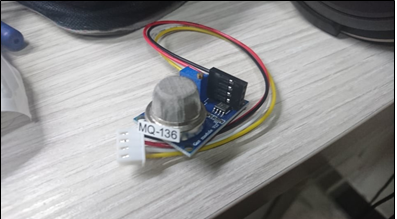
\includegraphics[width=0.5\textwidth]{pic/mq-136.png}
			\end{figure}
		\end{itemize}
		\item MQ-137 \begin{itemize}
			\item 對氨氣、三甲胺、乙醇胺氣體具有很高的靈敏度
			\item 在本實驗中用於測量氨氣濃度
			\begin{figure}[H]
				\centering
				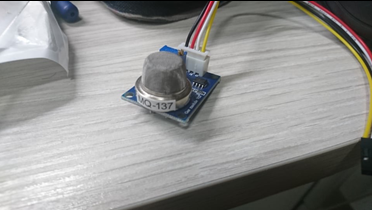
\includegraphics[width=0.5\textwidth]{pic/mq-137.png}
			\end{figure}
		\end{itemize}
		\item MH-Z19B \begin{itemize}
			\item 主要應用於暖通製冷與室內空氣品質監控
			\item 在本實驗用於測量二氧化碳濃度
			\begin{figure}[H]
				\centering
				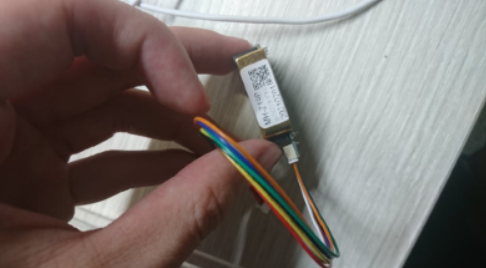
\includegraphics[width=0.5\textwidth]{pic/mh-z19B.png}
			\end{figure}
		\end{itemize}
	\end{itemize}
	\subsection{控制板}
	\begin{itemize}
		\item Arduino UNO R3:用於連接感測器,並執行感測器的相關讀取程式來取得需要的氣體濃度數據
		\begin{figure}[H]
			\centering
			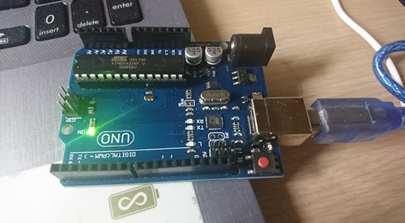
\includegraphics[width=0.5\textwidth]{pic/Uno.png}
		\end{figure}
	\end{itemize}
	\subsection{ML模型}
	\begin{itemize}
		\item 決策樹\footnote{\url{https://zh.wikipedia.org/wiki/决策树}}\\
			決策樹(英語:Decision tree)演算法採用一樹狀結構,透過一層一層的判斷來實現我們需要的分類。
			樹中每個節點表示某個特徵,而每個分叉路徑則代表某個特徵可能出現的屬性值,
			而每個葉節點則對應從根節點到該葉節點中間所經歷的路徑所表示的對象的值。
		\item KNN\footnote{\url{https://zh.wikipedia.org/zh-tw/K-近邻算法}}\\
			K-最近鄰居法(k-nearest neighbors algorithm),是一種預先設定要取 K 值,
			表示接下來要分 K 個群。接下來會依序將每個點判斷,放入不同的類別。每次判斷完,
			都會重新更新一個類別族群的資料,並繼續新的點的判斷分類。
		\item 單純貝氏\footnote{\url{https://zh.wikipedia.org/wiki/朴素贝叶斯分类器}}\\
			單純貝氏(英語:Naive Bayes)演算法是以貝氏定理為基礎,透過機率的計算,用以判斷未知類別的資料應該屬於那一個類別。
			概念是藉由分析資料中不同特徵與標籤之間發生的機率,並以此作為分類的依據。
		\item AdaBoost\footnote{\url{https://zh.wikipedia.org/wiki/AdaBoost}}\\
			自適應增強(英語:Adaptive Boosting,簡稱 AdaBoost)是一種迭代算法,在每一輪中加入一個新的弱分類器並更改資料的權重,
			直到達到某個預定的足夠小的錯誤率或迭代次數。每一個訓練樣本一開始都被賦予一個相同的權重,
			之後經過弱分類器分類後,已經被準確地分類的樣本權重會降低,反之錯誤的權重會增加,
			權重改變後資料集會被用於訓練下一個弱分類器,如此迭代地進行下去。
			最後將所有弱分類器組合成強分類器。各個弱分類器的訓練過程結束後,增加誤差率小的弱分類器的權重,
			反之降低誤差率大的弱分類器的權重,使其在最終的分類函數中起著較大的決定作用。
	\end{itemize}

	\chapter{研究結果}

\section{感測器檢測狀況}
(圖片)\\
使用的三個感測器皆已成功完成線路連接,且能及時讀取氣體濃度,但唯獨 MH-Z19B 重新啟動時需等待其熱機完畢方可使用。

\section{模型準確度}
\begin{itemize}
	\item 決策樹\\
	(圖片)\\
	\item SVM\\
	(圖片)\\
	\item 單純貝氏\\
	(圖片)\\
	\item AdaBoost\\
	(圖片)\\
\end{itemize}

\section{設備外型}
(圖片)\\
	\chapter{結論與心得}

	
	\nocite{*}
    	\linespread{1}\selectfont
    	\printbibliography[title=參考文獻]
    	\addcontentsline{toc}{chapter}{參考文獻}
\end{document}